\documentclass[12pt]{extarticle}
\usepackage[legalpaper, portrait, margin=2in]{geometry}
\usepackage{amsmath}
\usepackage{amssymb}
\usepackage{graphicx}
\graphicspath{{./Mini KSK Simulation Problems/}}

\usepackage{enumitem}
\renewcommand{\baselinestretch}{1.5}
\addtolength{\oddsidemargin}{-1in}
\addtolength{\evensidemargin}{-1in}
\addtolength{\textwidth}{2in}

\addtolength{\topmargin}{-1.2in}
\addtolength{\textheight}{2.5in} 

\title{Simulasi Kompetisi Sains Nasional Bidang Matematika SMA/MA Seleksi Tingkat Kota/Kabupaten Tahun 2021}
\author{120 menit}

\date{\today}

\begin{document}
	\maketitle
	
	\section{Kemampuan Dasar}
	Pada bagian ini setiap jawaban yang benar bernilai 2 poin dan setiap jawaban yang salah
	atau kosong bernilai nol.
	\begin{enumerate}
		
		
		\item Jika $a,b,c,d$ adalah bilangan asli berbeda sehingga $abcd=2020$, maka nilai terkecil yang mungkin dari $\dfrac{a+b}{c+d}$ adalah...
		
		\item Jumlah $n$ suku pertama suatu barisan aritmetika adalah 195. Jika suku pertama deret tersbut adalah $n$ dan suku ke-$n$ adalah 127, maka selisih barisan tersebut adalah...
		
		\item Perhatikan bangun seperempat lingkaran berikut. Jika $CA=6$ dan $ED+DF=8$, maka keliling yang diarsir adalah...
		
		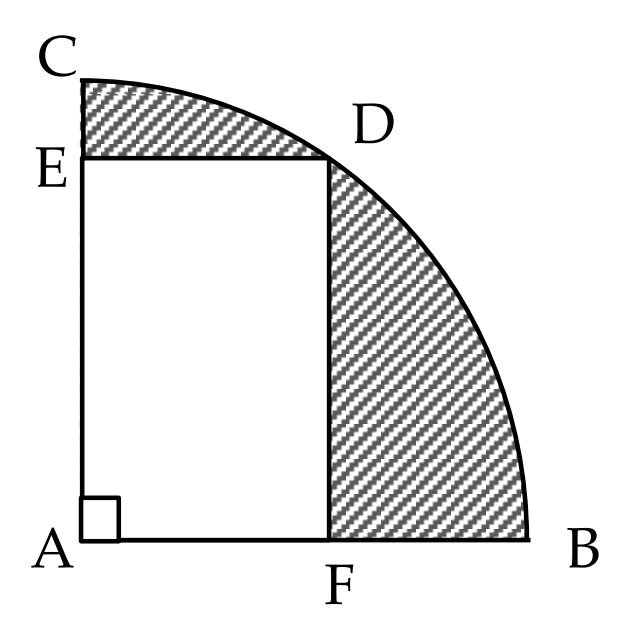
\includegraphics[scale=0.5]{simulasi1-1}
		
		\item Sebuah dadu seimbang enam sisi dilempar sebanyak $n$ kali. Jika rata-rata mata dadu yang keluar adalah $\frac{1}{4}n$, maka median dari seluruh nilai $n$ yang mungkin adalah...
		
		
		\item Jika $a,b$ adalah bilangan real positif yang memenuhi $a^{505}+b^{505}=1$, maka nilai minimum dari $a^{2020}+b^{2020}$ adalah...
		
		\item Diketahui segi delapan beraturan $ABCDEFGH$ yang mempunyai panjang sisi 2 cm. Misalkan $A$ adalah himpunan luas semua segitiga yang titik-titik sudutnya diambil dari delapan titik sudut segi delapan tersebut. Jika jumlah semua anggota $A$ adalah $(a+b\sqrt{2})$ cm$^2$, nilai $a+b$ adalah...
		
		\item Bilangan rasional $x=\frac{a}{b}$ terbesar sedemikian sehingga $\frac{5}{a}+20b < 2020$ merupakan kuadrat sempurna untuk suatu bilangan asli $a,b$ adalah...
		
		\item Pada suatu kotak terdapat 40 bola merah dan hijau. Dua bola diambil secara acak dan diamati warnanya. Jika peluang terambil kedua bola berwarna merah adalah $\frac{5}{12}$, maka banyaknya bola merah di dalam kotak semula adalah...
		
		\item Carilah seluruh pasangan bilangan bulat positif $(a,b,x)$ yang memenuhi $x^a+x^b=x^{a+b}$. 
		
		\item Carilah bentuk paling sederhana dari $\sqrt{104\sqrt{6}+468\sqrt{10}+144\sqrt{15}+2006}$.
		
	\end{enumerate}

\section{Kemampuan Lanjut}
Pada bagian ini setiap jawaban yang benar bernilai 4 poin, jawaban kosong bernilai nol
dan jawaban \textbf{salah} bernilai -1 (\textbf{minus satu})

\begin{enumerate}
		\item Untuk bilangan real positif $a,b,c$ yang memenuhi $$\frac{a}{a+1}+\frac{b}{b+1}+\frac{c}{c+1} = 1,$$ tentukan nilai maksimum dari $abc$.
		
		\item Azura sedang berada di toko ikan hias dan berniat membeli sepasang ikan koi. Penjaga toko membebaskan Azura untuk mengambil sepasang ikan tersebut dari suatu akuarium besar di tengah toko yang berisi $n>1$ ikan secara acak. Peluang Azura mendapatkan ikan dengan jenis kelamin yang sama adalah $\dfrac12$. Jika banyaknya ikan koi jantan sama dengan tiga kali banyak ikan koi betina, nilai minimum $n$ adalah...
		
		\item Carilah seluruh bilangan bulat positif terkecil yang memenuhi $x^2+x+1 \equiv 0 \mod 49$
		
		\item Misalkan suatu lingkaran mempunyai diameter $AB$ dan $P$ sebagai titik di luar lingkaran tersebut. Garis $PQ$ dan $PR$ menyinggung lingkaran di $Q$ dan $R$. Garis $PH$ berpotongan tegak lurus dengan garis $AB$ di $H$ dan $PH$ berpotongan dengan $AR$ di $S$. Jika $\angle QPH = 40^\circ$ dan $\angle QSA = 30^\circ$, tentukan besar $\angle RPS$.
		
		\item Berapa banyak bilangan real $x$ yang memenuhi $\sqrt[4]{x+15} = \sqrt[3]{x}+1$ ?
		
		\item  Terdapat sebuah rapat yang terdiri dari 40 kursi yang dihadiri oleh 16 tamu undangan.
		Untuk menghindari penularan COVID-19, maka setiap tamu undangan harus dibatasi minimal
		dengan 1 kursi. Tentukan banyaknya susunan mereka duduk.

		
		\item Pada ekspresi $$a= \sqrt{2020+\sqrt{2020+\sqrt{2020+\sqrt{2020+...}}}}$$
		bilangan 2020 muncul sebanyak 1442 kali di dalam akar. Tentukan nilai $\left \lceil a \right \rceil$.
		
		\item Misalkan $ABC$ adalah segitiga dengan $AB=9, BC=20,$ dan $CA=16$. Titik $D$ terletak pada segmen $BC$ sehingga $DB=DA$. Garis bagi luar $\angle BAC$ memotong perpanjangan $BC$ di $E$. Misalkan $F$ adalah titik tengah $DE$. Tentukan panjang $FA$.
		
		\item Untuk sebarang bilangan asli $n \ge 2$, misalkan $A_n$ adalah himpunan semua solusi persamaan $$x=\left\lfloor \frac{x}{2}\right \rfloor+\left\lfloor \frac{x}{3}\right \rfloor+\dots+\left\lfloor\frac{x}{n} \right \rfloor.$$
		
		Jika $S = A_2 \cup A_3 \cup A_4 \cup \dots \cup A_n$, tentukan nilai dari elemen terbesar $S$.
		
		\item Misalkan $ABCD$ adalah segiempat tali busur. Diagonal $AC$ dan $BD$ berpotongan di titik $E$. Jika $BD=24$, tentukan nilai minimum dari $\dfrac{1}{AE}+\dfrac{1}{EC}$.
		
\end{enumerate}
\end{document}